\documentclass{article}
\usepackage[utf8]{inputenc}
\usepackage[UKenglish]{babel}
% \usepackage{fontspec}
% \usepackage{polyglossia}
% \usepackage{unicode-math}
\usepackage{minted}
\usepackage{listings}
\usepackage{xcolor}
\usepackage{quiver}
\usepackage[pdf]{graphviz}
\usepackage{caption, subcaption}

\definecolor{codegreen}{rgb}{0,0.6,0}
\definecolor{codegray}{rgb}{0.5,0.5,0.5}
\definecolor{codepurple}{rgb}{0.58,0,0.82}
\definecolor{backcolour}{rgb}{0.95,0.95,0.92}
\lstdefinestyle{mystyle}{
    backgroundcolor=\color{backcolour},
    commentstyle=\color{codegreen},
    keywordstyle=\color{magenta},
    numberstyle=\tiny\color{codegray},
    stringstyle=\color{codepurple},
    basicstyle=\ttfamily\footnotesize,
    breakatwhitespace=false,
    breaklines=true,
    captionpos=b,
    keepspaces=true,
    numbers=left,
    numbersep=5pt,
    showspaces=false,
    showstringspaces=false,
    showtabs=false,
    tabsize=2
}

\lstset{style=mystyle}

\usepackage{tabularx}
\usepackage{booktabs}
\renewcommand{\arraystretch}{1.5}

\usepackage{mathtools}
\setcounter{MaxMatrixCols}{20}
\usepackage{enumitem}
\setenumerate[0]{label=(\arabic*)}

\usepackage[linesnumbered,ruled,vlined]{algorithm2e}
\newcommand\mycommfont[1]{\footnotesize\ttfamily\textcolor{blue}{#1}}
\SetCommentSty{mycommfont}

\SetKwInput{KwInput}{Input}                % Set the Input
\SetKwInput{KwOutput}{Output}              % set the Output


% Kan Danny godt lide!
\usepackage[autostyle]{csquotes}
\usepackage{kpfonts}
\usepackage{inconsolata}
\linespread{1.06}

\usepackage{xcolor}
\usepackage{hyperref}
\hypersetup{%
	pdftitle=Reinforcement learning for mathematical applications,
	pdfauthor={Andreas Bøgh Poulsen},
	colorlinks,
	linkcolor={red!50!black},
	citecolor={red!50!black},
	urlcolor={red!50!black},
	bookmarksnumbered=true
}

\usepackage[ntheorem]{mdframed}
\usepackage[amsmath,thmmarks,hyperref]{ntheorem}
\usepackage[capitalize]{cleveref}

% Frame for theorems
\definecolor{shadecolor}{gray}{0.93}
\definecolor{rulecolor}{gray}{0.4}
\mdfdefinestyle{thmframed}{%
	%usetwoside=false, % For use with memoir twoside
	skipabove=0.5em plus 0.4em minus 0.2em,
	skipbelow=0.5em plus 0.4em minus 0.2em,
	leftmargin=-7pt, rightmargin=-7pt, innerleftmargin=6pt,
	innerrightmargin=6pt, innertopmargin=6pt, innerbottommargin=3pt,
	linewidth=1pt, linecolor=rulecolor, backgroundcolor=shadecolor,
	splittopskip=1.2em minus 0.2em,
	splitbottomskip=0.5em plus 0.2em minus 0.1em,
}

% New theorem style with a dot
\makeatletter
\newtheoremstyle{changedot}%
  {\item[\hskip\labelsep \theorem@headerfont ##2~~$\cdot$~~##1\theorem@separator]}%
  {\item[\hskip\labelsep \theorem@headerfont ##2~~$\cdot$~~##1\ (##3)\theorem@separator]}

\newtheoremstyle{changedotbreak}%
  {\item\hbox to \textwidth{\theorem@headerfont ##2~~$\cdot$~~##1\theorem@separator\hfill}}%
  {\item\hbox to \textwidth{\theorem@headerfont ##2~~$\cdot$~~##1\
      (##3)\theorem@separator\hfill}}
\makeatother

\theoremstyle{changedot}
\theoremseparator{.}
\newmdtheoremenv[style=thmframed]{theorem}{Theorem}[section]
\newmdtheoremenv[style=thmframed]{proposition}[theorem]{Proposition}
\newmdtheoremenv[style=thmframed]{lemma}[theorem]{Lemma}
\newmdtheoremenv[style=thmframed]{corollary}[theorem]{Corollary}

\theorembodyfont{\normalfont}
%\theoremsymbol{\ensuremath{\triangle}}
\newmdtheoremenv[style=thmframed]{definition}[theorem]{Definition}

\theoremstyle{changedotbreak}
\newmdtheoremenv[style=thmframed]{definitionbreak}[theorem]{Definition}

\theoremstyle{nonumberplain}
\theoremheaderfont{\normalfont\itshape}
\theorembodyfont{\normalfont}
\theoremsymbol{\ensuremath{\square}}
\newtheorem{proof}{Proof}
\newtheorem{remark}{Remark}
\newtheorem{example}{Example}

\Crefname{theorem}{Theorem}{Theorems}
\Crefname{proposition}{Proposition}{Propositions}
\Crefname{lemma}{Lemma}{Lemmata}
\Crefname{corollary}{Corollary}{Corollaries}
\Crefname{definition}{Definition}{Definitions}

\crefformat{equation}{(#2#1#3)}

% / Kan Danny godt lide

% Kan Andreas godt lide
\setlength{\parindent}{1em}
\setlength{\parskip}{0.7em}


\title{Reinforcement learning for mathematical applications}
\author{
    Andreas Bøgh Poulsen\\
    201805425
}
% \date{28th June 2020}


\usepackage{csquotes}
\usepackage[backend=biber, style=alphabetic, maxcitenames=1]{biblatex}
\addbibresource{references.bib}

\usepackage{microtype}

\usepackage{graphicx}




\newcommand{\ro}[1]{^{\setminus #1}}
\newcommand{\rr}  {^{\setminus}}

\DeclarePairedDelimiter{\tuple}{\langle}{\rangle}
\newcommand{\calM}{\mathcal{M}}
\newcommand{\calV}{\mathcal{V}}
\newcommand{\calD}{\mathcal{D}}
\newcommand{\calG}{\mathcal{G}}

\newcommand{\m}{\mathbb}

\newcommand{\true}{\textsc{true}}
\newcommand{\false}{\textsc{false}}

\DeclareMathOperator{\lcm}{lcm}

\DeclareMathOperator*{\smallbigcup}{\textstyle\bigcup}
\DeclareMathOperator*{\bigunion}{\mathchoice
	{\smallbigcup}%
	{\bigcup}%
	{\bigcup}%
	{\bigcup}%
}
\DeclareMathOperator*{\smallbigcap}{\textstyle\bigcap}
\DeclareMathOperator*{\bigintersect}{\mathchoice
	{\smallbigcap}%
	{\bigcup}%
	{\bigcup}%
	{\bigcup}%
}

\DeclarePairedDelimiter{\abs}{\lvert}{\rvert}
\DeclarePairedDelimiter{\norm}{\lVert}{\rVert}

\newcommand{\setN}{\mathbb{N}}
\newcommand{\setR}{\mathbb{R}}
\newcommand{\card}[1]{\abs{#1}}

\let\phi\varphi
\frenchspacing

% Partial functions
% From https://tex.stackexchange.com/questions/47142/how-to-tex-an-arrow-with-vertical-stroke

\makeatletter
\newcommand{\pto}{}% just for safety
\newcommand{\pgets}{}% just for safety

\DeclareRobustCommand{\pto}{\mathrel{\mathpalette\p@to@gets\to}}
\DeclareRobustCommand{\pgets}{\mathrel{\mathpalette\p@to@gets\gets}}

\newcommand{\p@to@gets}[2]{%
  \ooalign{\hidewidth$\m@th#1\mapstochar\mkern5mu$\hidewidth\cr$\m@th#1\to$\cr}%
}
\makeatother

\newcommand{\id}{\mathrm{id}}
\DeclarePairedDelimiter{\ceil}{\lceil}{\rceil}
\DeclarePairedDelimiter{\floor}{\lfloor}{\rfloor}
\DeclarePairedDelimiter{\anglemap}{\langle}{\rangle_{\infty}}

\newcommand{\nextk}{\mathrm{next}}
\newcommand{\enc}{\mathrm{enc}}

\newcommand{\binlit}[1]{\mathbf{#1}}
\newcommand{\bin}{\mathrm{bin}}
\newcommand{\val}{\mathrm{val}}
\newcommand{\Seq}{\mathrm{Seq}}
\newcommand{\length}[1]{\abs{#1}}

\DeclarePairedDelimiter{\gpath}{\langle}{\rangle}


\begin{document}

\maketitle

\section{Introduction}
In 2020 Dylan Peifer et al\cite{peifer} showed how to use deep learning to improve the performance of algorithms for constructing Gröbner bases. The goal of this project was to reproduce the results of this paper, as well as attempt some other techniques.

The structure of this report is as follows: first, we'll discuss the use of reinforcement learning, a branch of deep learning used by Peifer et al. We'll cover both the conceptual framework, as well as two particular techniques: Q-learning and policy gradients. Next, a brief overview of Gröner bases, their uses and how to compute them. Third part covers our experimental results featuring both an evaluation of existing heuristics as well as our results.

\section{Gröbner bases}

Since the problem we're considering is the construction of Gröbner bases, let's give a short introduction to Gröbner bases.

We fix a field $k$ and consider the polynomial ring $R = k[x_{1}, \dots, x_{n}]$. For at set of polynomials $F = \{f_{1}, \dots, f_{l}\}$ we consider the ideal $I = \tuple{f_{1}, \dots, f_{l}}$ generated by these polynomials. Now, we wish to efficiently determine whether a given polynomial $f$ lies in $I$ or not. We know that $R$ is a \emph{unique factorization domain} so it is decidable, but giving an efficient algorithm is tricky. Instead, we extend the generating set of the ideal in a way that doesn't change the ideal but gives us stronger properties, enabling an efficient desicion algorithm.

Fix a \emph{term order} which is a well-order relation $>$ on $\mathbb N^{n}$ such that $a > b$ implies $a + c > b + c$ for any $a, b, c \in \mathbb N^{n}$. This naturally extends to a so called \emph{monomial order} on monomials $\{x^{v} = x_{1}^{v_{1}} \cdots x_{n}^{v_{n}} \mid v \in \mathbb N^{n}\}$ by comparing exponent vectors of the monomials. We'll write $>$ for both orders.

There are two common term orders: lexicographic and grevlex. Lexicographic has $a > b$ if there exists $k$ s.t. $a_{i} = b_{i}$ for $i < k$ and $a_{k} > b_{k}$. This is the usual ``alphabetix order'' on tuples. Grevlex ordering is often used in implementations using Gröbner bases and has $a > b$ if $\sum_{i} a_{i} > \sum_{j} b_{j}$ or   $\sum_{i} a_{i} = \sum_{j} b_{j}$ and the last non-zero entry of $a - b$ is negative.

Given a monomial order we can define the \emph{initial term} and the S-polynomial.

\begin{definition}
  Given a monomial order $>$, the \emph{initial term} of a polynomial $f = \sum_{v} \lambda_{v} x^{v}$, denoted $in_{>}(f)$ is the greatest term of $f$ with respect to $>$. We will often omit the subscript when the order is either clear from context or arbitrary.
\end{definition}


Now, a naive division algorithm would look like this:

\begin{algorithm}[H]
\DontPrintSemicolon

  \KwInput{Polynomial $f$ and $F = \{f_{1}, \dots, f_{l}\}$}
  \KwOutput{Remainder $r$ s.t. $f - r \in \tuple F$ and $in(f_{i}) \nmid in(r)$ for all $f_{i} \in F$}
  $r \leftarrow f$\;
  \While{$\exists i. in(f_{i}) \mid in(r)$}
    {
        $r \leftarrow r - \frac{in(r)}{in(f_{i})} f_{i}$
    }

    \caption{Division algorithm $reduce(f, F)$}
    \label{alg:div}
\end{algorithm}

This algorithm terminates since the initial term of $r$ is strictly descreasing with respect to $>$. However, this algorithm has some problems. In particular, we do not always get that $reduce(f, F) = 0$ when $f$ lies in the ideal generated by $F$, as we would expect. This is due to the choice of which polynomial to reduce with in line 3.

An example where this does not hold without a Gröbner basis is \colorbox{red}{example 5.4.3 in NL}.

Now, we're ready to present Gröbner bases and the theorem that makes them so important:

\begin{definition}
  A Gröbner basis for an ideal $I$ is a set of polynomials $F = \{f_{1}, \dots, f_{l}\} \subseteq I$ such that $in(f_{i}) \mid in(f)$ for all $f \in I\setminus \{0\}$.

  Note that this implies $\tuple F = I$.
\end{definition}

\begin{theorem}
  Let $G = \{f_{1}, \dots, f_{l}\}$ be a Gröbner basis for an ideal $I$. Then $reduce(f, G) = 0 \Longleftrightarrow f \in I$.
\end{theorem}
\begin{proof}
  If $reduce(f, G) = 0$ then $f = f - 0 \in I$.

  If $f \in I$ and $f - r = h \in I$ then $r = f - h \in I$. But as guaranteed by the division algorithm, there is no $f_{i} \in G$ where $in(f_{i}) \mid in(r)$ even though $G$ is a Gröbner basis. The only element in $I$ not subject to the Gröbner basis constraint is zero, thus $r$ must be zero.
\end{proof}

So, Gröbner bases are great, but how do we construct them? Do they even exist for every ideal? They do exist and we have an algorithm called Buchbergers algorithm to find them, bt first we need a construction called the S-polynomial or syzygy polynomial.

\begin{definition}
  The S-polynomial of two polynomials $f$ and $g$ is denoted $S(f, g) = \frac{x^{w}}{in(f)} f - \frac{x^{w}}{in(g)} g$ where $x^{w} = lcm(in(f), in(g))$ is a least common multiple of $f$ and $g$.
\end{definition}

The Buchberger criterion is a simple was to check if we have a Gröbner basis, and it even leads us to an algorithm for constructing Gröbner bases.

\begin{theorem}\label{thm:buchberger_crit}
Let $F = \{f_{1}, \dots, f_{l}\}$ be a set of polynomials and let $I = \tuple F$ be the ideal generated by $F$. If $\text{reduce}(S(f_{i}, f_{j}), F) = 0$ for all $f_{i}, f_{j} \in F$ then $F$ is a Gröbner basis for $I$.
\end{theorem}
\begin{proof}
  See appendix.
\end{proof}

We can now present the Buchberger algorithm:

\begin{algorithm}[H]
\DontPrintSemicolon

  \KwInput{A set of polynomials $F = \{f_{1}, \dots, f_{l}\}$}
  \KwOutput{A Gröbner basis $G$ of the ideal $I = \tuple F$}
  $G \leftarrow F$ \;
  $P \leftarrow \{(f_{i}, f_{j}) \mid 1 \leq i < j \leq l\}$ \;
  \While{$|P| > 0$}
  {
    $(g, h) \leftarrow \text{select}(P)$ \;
    $P \leftarrow P \setminus \{(g, h)\}$ \;
    $r \leftarrow \text{reduce}(S(g, h), G)$ \;
    \If{$r \neq 0$}
    {
      $P \leftarrow \text{update}(P, G, r)$ \;
      $G \leftarrow G \cup \{r\}$ \;
    }
  }

\caption{Buchbergers algorithm}
\end{algorithm}

Notice that the algorithm uses 2 routines we haven't defined: \emph{select} and \emph{update}. The simplest implementations are $\text{select( $P$ )} = P_{1}$ taking the first pair in $P$ and $\text{update( $P, G, r$ )} = P \cup \{(f, r) \mid f \in G\}$.

Buchbergers algorithm adds remainders of syzygy polynomials until they all reduce to 0. Keeping theorem \ref{thm:buchberger_crit} in mind, it is clear that $G$ will be a Gröbner basis when the algorithm terminates.

To produce a faster version of Buchbergers algorithm, these two routines are good places to start. During \emph{update} we can eliminate a large number of pairs using simpler criteria than theorem \ref{thm:buchberger_crit}. We'll discuss a better version in section \ref{sec:update}.

The problem of selecting the next pair of polynomials is not easy and it turns out to have serious consequences. Simply switching from taking the first pair to taking the last one, i.e. treating $P$ as a stack instead of a queue, can reduce the number of polynomial additions by almost 50\%.

There are a number of standard selection strategies:

\begin{itemize}
  \item[Random] Pick a random pair uniformly.

  \item[First] Pick the lexicographically smallest pair, where the order of polynomials is given by their order in $G$.

  \item[Queue] Treat $P$ as a queue and select the pair that was added first.

  \item[Stack] Treat $P$ as a stack and select the pair that was most recently added.

  \item[Degree] Pick the pair $(f, g)$ with the smallest total degree of $lcm(in(f), in(g))$.

  \item[Normal] Pick the pair $(f, g)$ where $lcm(in(f), in(g))$ is smallest in the used monomial order.

  \item[Sugar] Pick the paie $(f, g)$ with the smallest \emph{sugar degree} which is the degree $S(f, g)$ woudl have had, if the polynomials had been homogenized.

  \item[TrueDegree] Introduced in \cite{peifer}, pick the pair $(f, g)$ whose S-polynomial has the lowest degree.
\end{itemize}


\subsection{A better \emph{update}}  \label{sec:update}
In the Buchberger algorithm, a pair $(f, g)$ will be removed if $\text{reduce}(S(f, g), G) = 0$. However, this is computationally expensive test. Fortunately, there are some easier tests that can eliminate a large number of pairs. I'll describe the tests described in Gebauer \& Möller.

\subsubsection{Operational description}
Gebauer \& Möller reduction is performed as part of the procedure $\text{update}(P, G, r)$. First, in the pair set $P$ we remove every pair $(f, g)$ where $in(r) | \lcm(in(f), in(g))$ and $\lcm(in(f), in(r)) \neq \lcm(in(f), in(g)) \neq \lcm(in(g), in(r))$.

Next, consider the set $P' = \{(f, r) \mid f \in G\}$. These are all the pairs we should naively add to $P$. Partition $P'$ into equivalence classes using the equivalence realation $(f, r) \sim (g, r) \Longleftrightarrow \lcm(in(f), in(r)) = \lcm(in(g), in(r))$. Remove every equivalence class containing no element $(f, r)$ satisfying $\lcm(in(f), in(r)) = in(f) in(r)$ and take a representative from each remaining equivalence class. Let $P''$ be this set of representatives and let $P \cup P''$ be the result of $\text{update}(P, G, r)$.


\subsubsection{Justification and proof}
Simply put, Gebaur\& Möller reduction consists of reducing a Gröbner basis. Once a Gröbner basis is constructed, we may throw our any redundant element. This process is described above and the proof that this maintains the Gröbner basis property can be found in \cite{NL} section 5.8.

For the setup we need to extend the concept of Gröbner bases to free modules over a polynomial ring. R be a multinomial ring in $n$ variables over a field $k$ and $e_{1}, \dots, e_{m}$ be the canonical basis of $R^{m}$. Since every element of $R^{m}$ is a $k$-linear combination of elements of the form $x^{v}e_{i}$, $v \in \m N^{n}$, we call these $x^{v}e_{i}$ for monomials. Now, the definition of Gröbner bases require two more parts: a monomial order and a divisability test. Monomial orders work the same way, they're a total order satisfying \[x^{v_{1}}e_i < x^{v_{2}}e_{j} \Longrightarrow x^{v_{1} + v} e_{i} < x^{v_{2} + v} e_{j}\] for all $v \in \m N^{n}$. We say that $x^{v_{1}}e_{i}$ divides $x^{v_{2}}e_{j}$ iff $i=j$ and $x^{v_{1}}$ divides $x^{v_{2}}$. Now, the definition of a Gröbner basis is the same, and we will repeat it here: a Gröbner basis for a submodule $M \subset R^{m}$ is a set of elements $F = \{m_{1}, \dots, m_{t}\} \subset M$ such that $in(m_{i})$ divides $in(m)$ for all $m \in M \setminus \{0\}$.

Now, consider the ideal of monomials $I = \tuple{x^{v_{1}}, \dots, x^{v_{m}}} \subset R$ and the natural surjection $p : R^{m} \to I$ sending $e_{i}$ to $x^{v_{i}}$. Now, let $K$ be the kernel of $p$ and notice that the syzygies in $I$ are a basis of $K$.

\begin{example}
If $I = \tuple{x, y, z}$ then $K$ will have a basis consisting of the syzygies $\{x e_{2} - y e_{1}, x e_{3} - x e_{1}, y e_{3} - z e_{2}\}$.
\end{example}

More generally, the elements \[S_{ij} = x^{\lcm(v_{i}, v_{j}) - v_{j}} e_{j} - x^{\lcm(v_{i}, v_{j}) - v_{i}} e_{i}, \, \, 1 \leq i < j \leq m\] are basis elements of $K$. However, this basis is usually not minimal. Now, we need two propositions, the first due to Schreyer.

\begin{theorem}
 There exists a monomial order called the Schreyer order such that set $\{S_{ij} \mid 1 \leq i < j \leq m\}$ is a Gröbner basis for $K$ over this order.
\end{theorem}

The second is proposition 2.9.9 from \cite{IVA}.

\begin{theorem}
  Let $G = \{g_{1}, \dots, g_{m}\}$ be a basis for an ideal $I$. Then $G$ is a Gröbner basis for $I$ iff for every basis element of the syzygies of G $S = \sum_{i = 1}^{m} x^{u_{i}} e_{i}$ we have $\sum_{i=1}^{m} x^{u_{i}} g_{i} \to_{G} 0$.
\end{theorem}

Now, this is a refinement of the Buchberger S-criterion. It is therefor enough to reduce the S-pairs corresponding to any Gröbner basis of the syzygies. In particular, we may take the basis $\{S_{ij} \mid 1 \leq i < j \leq m\}$ and reduce it to a minimal Gröbner basis before reducing mod $G$ and adding to $G$.


\section{Abstract framework of deep learning}

We would like to use modern advances in machine learning to learn a better selection strategy for Buchbergers algorithm. However, to do so we need some machinery. Since we need to use the \emph{select}-function multiple times, we need to use a branch of machine learning called \emph{reinforcement learning}.

\subsection{Reinforcement-learning and Markov Decision Processes}

Constructing Gobner bases can be seen as an interaction between an agent and an environment: we pick a pair to reduce, perform polynomial reduction, add some new pairs to the set of pairs and go again. We want to do the least amount of work when we're done. This interaction can be modeled using Markov decision processes.

A Markov decision process (MPD for short) is an interaction between an environment and an agent. At timestep $t = 0, 1, 2, \dots$ the agent recieves a \emph{state}, $S_{t}$ and selects an \emph{action}, $a_{t}$. The agent then recives a \emph{reward}, $r_{t+1}$ and a new state $s_{t+1}$ and the process repeats.

% https://q.uiver.app/?q=WzAsMixbMCwwLCJcXHRleHR7QWdlbnR9Il0sWzAsMiwiXFx0ZXh0e0Vudmlyb25tZW50fSJdLFswLDEsIlxcdGV4dHthY3Rpb259IFxcXFwgYV90IiwwLHsib2Zmc2V0IjotMSwiY3VydmUiOi01fV0sWzEsMCwiXFx0ZXh0e3N0YXRlfSBcXFxcIHNfdCIsMCx7Im9mZnNldCI6LTUsImN1cnZlIjotNX1dLFsxLDAsIlxcdGV4dHtyZXdhcmR9IFxcXFwgcl90IiwyLHsiY3VydmUiOi01fV1d
\[\begin{tikzcd}
	{\text{Agent}} \\
	\\
	{\text{Environment}}
	\arrow["{\text{action: } \\ a_t}", shift left=1, curve={height=-30pt}, from=1-1, to=3-1]
	\arrow["{\text{state: } \\ s_t}", shift left=5, curve={height=-30pt}, from=3-1, to=1-1]
	\arrow["{\text{reward: } \\ r_t}"', curve={height=-30pt}, from=3-1, to=1-1]
\end{tikzcd}\]

This gives rise to a \emph{trajectory} which looks like this:

\[\tau = s_{0}, a_{0}, r_{1}, s_{1}, a_{1}, r_{2}, s_{2}, a_{2}, \dots\]

We'll sometimes denote $\tau_{p} = s_{p}, a_{p}, r_{p+1}, s_{p+1}, \dots$.

Formally, this can be described in terms of the following definition:

\begin{definition}
  \emph{Environment and policy}
  \begin{itemize}
      \item Fix two non-empty, finite sets $S$ and $R \subset \m R$ and a family of non-empty finite sets $A_{s}$ for all $s \in S$. We call $S$ the \emph{state-space}, $A_{s}$ an \emph{action-space} and $R$ the \emph{reward space}. Then an \emph{environment} is a probability distribution \[p(s', r \mid s, a) = P(s_{t+1} = s', r_{t+1} = r \mid s_{t} = s, a_{t} = a)\] for all $s, s' \in S$, $r \in R$ and $a \in A(s)$.

      \item Given an environment, an \emph{policy} is a propability distribution $\pi(a \mid s)$ of taking an action $a$ given a state $s$.
  \end{itemize}
\end{definition}

An important property of a MPD is that the probability of $s_{t}$ depends only on $s_{t-1}$ and $a_{t-1}$, not all of the earlier states and actions. Do also note, that we can derive marginal probabilities from the $p-function$, for example the probability of reaching a certain state \[p(s' \mid s, a) = P(s_{t+1} = s' \mid s_{t} = s, a_{t} = a) = \sum_{r \in R} p(s', r \mid s, a).\]

Now, an agent can interact with an environment by choosing actions and revieving rewards. Such an interation leads to a trajectory $\tau = s_{0}, a_{0}, r_{1}, s_{1}, a_{1}, r_{2}, s_{2}, a_{2}, \dots$. We're interested in minimizing the total reward of the trajectory or the \emph{return} \[G(\tau) := \sum_{t=1}^{\infty} \gamma^{t} r_{t}\] where $0 < \gamma < 1$ is put in place to ensure convergence of the infinite series. However, if the rewards are eventually always zero, we may choose $\gamma = 1$. Usually a value around 0.99 is chosen for $\gamma$.

\subsection{Pair selection as a Markov Decision Process}
The problem of pair selection is modeled as a Markov Decision Process. During a run of Buchbergers Algorithm the \emph{select} subroutine is implemented by the agent. At timestep $t$ the agent sees the state $P_{t}$ which is the current set of polynomial pairs. The agent must then choose a pair $a_{t} \in P_{t}$ which is fed back into Buchbergers algorithm as the result of \emph{select}. The environment then updates by removing $p$ from $P$, reducing the correpsonding and S-polynomial and updating $G$ and $P$.

The reward $r_{t}$ given for the action $a_{t}$ is $-1$ times the number of polynomial additions performed when reducing $a_{t}$. This metric is chosen since it is the most expensive computation and it serves as a proxy for total computation.

This loops until a complete Gröbner basis is constructed at timestep $T$, yielding the trajectory $\tau = (P_{0}, a_{0}, r_{0}, \dots, P_{T}, a_{T}, r_{T})$. The goal of the agent is to maximize the exprected return $\m E[\sum_{t=1}^{T} r_{t}]$ which is minimizing the number of polynomial additions.

It is not immidiately obvious that the state-space is finite. However, the running time of Buchbergers algorithm has been shown to be worst-case $d^{2^{n+\mathcal{O}(1)}}$ where $n$ is the number of variables and $d$ is the maximum total degree of any generator. This means the set $P$ of polynomial pairs can at most grow that large. Since at any step there is a finite number of actions and the algorithm terminates after a bounded number of actions, the number of possible states is finite. It's very large, but finite.

\section{Learning strategies}
The abstract framework of Markov Decision Processes is a rather simple idea. And indeed, that is not where the magic of reinforcement learning is. Reinforcement learning solves the challenge of credit assignment. We have sampled some trajectories, some leading to a high reward and some to a lower reward. How do we know what actions were responsible for the high rewards? How should we update the agent to increase the future rewards? In this section we'll describe two approaches: value estimation and policy gradients as well as some standard ``tricks'' that are used to improve performance.

\subsection{Value-estimation and Q-learning}
Most classical reinforcement learning is about estimating value functions -- how good a state or action is. For example, we can define the \emph{value} of a state $s$ given an agent $\pi$ to be \[v_{\pi}(s) = \mathbb E \left[ G(\tau_{p}) \mid s_{p} = s, \pi \right] = \m E \left[ \sum_{k=p}^{T} \gamma^{k} r_{k} \mid s_{p} = s, \pi \right].\] Here we sample the actions $a_{t}$ from the probability distribution given by $\pi$.

The value-function can be expressed recursively:
\begin{align}
  v_{\pi}(s) &= \m E[G(\tau_{p}) \mid s_{p} = s, \pi] \\
             &= \m E\left[ \sum_{k=p}^{T} \gamma^{k} r_{k} \mid s_{p} = s, \pi \right] \\
  &= \m E \left[ r_{p} + \gamma G(\tau_{p+1}), \mid s_{p} = s, \pi \right]
\end{align}

Now, we can further use the law of total probality twice to get
\begin{align}
  v_{\pi}(s) &= \m E[r_{p} + \gamma G(\tau_{p+1}) \mid s_{p} = s] \\
             &= \sum_{a} \pi(a \mid s) \m E[r_{p} + \gamma G(\tau_{p+1}) \mid s_{p} = s] \\
             &= \sum_{a} \pi(a \mid s) \sum_{s', r} p(s', r \mid s, a) \m E[r + \gamma G(\tau_{p+1}) \mid s_{p+1} = s'] \\
             &= \sum_{a} \pi(a \mid s) \sum_{s', r} p(s', r \mid s, a) ( r + \gamma \m E[G(\tau_{p+1}) \mid s_{p+1} = s'] )\\
             &= \sum_{a} \pi(a \mid s) \sum_{s', r} p(s', r \mid s, a) (r + \gamma v_{\pi}(s'))
\end{align}

And this actually gives us a way to learn. By starting with a random policy $\pi_{0}$ we can sample some trajectories, giving us values for $r, a$ and $s$. Then the above is a number of linear equations that can be solved to find $v_{\pi_{0}}(s)$ for every $s$. Based on this value-function we can devise a new strategy $\pi_{1}$ which chooses the action leading to the most valuable state. Repeating this process, called policy iteration in the literature, should provide better and better agents. It does work, but it has some serious limitations. An obvious one is in the face of non-deterministic environments: how do we know which state each action will lead to? That requires a good model of the environment to answer, which we may not have.

One solution to the problem above is to shift our focus slightly to consider the value of \emph{actions} instead of states. We can define an \emph{action-value} function, denoted \[q_{\pi}(s, a) = \m E[G(\tau_{p}) \mid s_{p} = s, a_{p} = a, \pi]. \]

Using these we can define the \emph{optimal} value functions:

\begin{definition}
  \[v_{*}(s) = \max_{\pi} v_{\pi}(s)\] is called the \emph{optimal value function} and \[q_{*}(s, a) = \max_{\pi} q_{\pi}(s, a)\] is called the \emph{optimal action-value function}
\end{definition}

These two functions can be expressed in terms of each other:
\begin{align*}
  v_{*}(s) &= \max_{\pi} v_{\pi}(s) \\
           &= \max_{\pi} \m E[G(\tau_{p} \mid s_{p} = s, \pi)] \\
           &= \max_{\pi} \sum_{a} \pi(a \mid s) \, \m E[G(\tau_{p}) \mid s_{p} = s, a_{p} = a, \pi] \\
           &= \max_{\pi} \sum_{a} \pi(a \mid s) \, q_{\pi} (s, a) \\
  &= \max_{a} q_{*}(s, a)
\end{align*}
and similarly we can get \[q_{*}(s, a) = R(s, a) + v_{*}(s').\] These of course also satisfies the recursive relations from before:
\begin{align*}
  v_{*}(s) &= \max_{a} q_{*}(s, a) \\
           &= \max_{a} \m E[G(\tau_{p}) \mid s_{p} = s, a_{p} = a, \pi_{*}] \\
           &= \max_{a} \m E[r_{p} + \gamma v_{*}(s_{p+1}) \mid s_{p} = a, a_{p} = a, \pi_{*}] \\
           &= \max_{a} \sum_{s', r} p(s' \mid s, a) (r + \gamma v_{*}(s') )
\end{align*}
which is called the Bellman equation for $v_{*}$. The Bellman equation for $q_{*}$ is
\[q_{*}(s, a) = \sum_{s', r} p(s', r \mid s, a) (r + \gamma \max_{a'} q_{*}(s', a')).\]

These equations inspires the learning equation
\[Q(s_{p}, a_{p}) = (1 - \alpha) Q(s_{p}, a_{p}) + \alpha (r_{p+1} + \gamma \max_{a} Q(s_{p+1}, a))\]

Here, $\alpha$ is called the learning rate. This is a slight variation of policy iteration, but whereas policy iteration worked on the state-value function, this equation applies to the action-value function as well. It can be shown that under light assumptions this learning method converges to the optimal q-function, for at full exposition see \cite{cjch}.


\begin{example}
  \begin{figure}
    % https://q.uiver.app/?q=WzAsMyxbMCwwLCJcXGJveGVke0F9Il0sWzIsMCwiXFxib3hlZHtCfSJdLFsxLDIsIlxcYm94ZWR7Q30iXSxbMCwxLCIxNSIsMCx7ImN1cnZlIjotMX1dLFsxLDAsIjMiLDAseyJjdXJ2ZSI6LTF9XSxbMSwyLCIxIiwwLHsiY3VydmUiOi0xfV0sWzIsMSwiOCIsMCx7ImN1cnZlIjotMX1dLFsyLDAsIjUiLDJdXQ==
    \[\begin{tikzcd}
        {\boxed{A}} && {\boxed{B}} \\
        \\
        & {\boxed{C}}
        \arrow["15", curve={height=-6pt}, from=1-1, to=1-3]
        \arrow["3", curve={height=-6pt}, from=1-3, to=1-1]
        \arrow["1", curve={height=-6pt}, from=1-3, to=3-2]
        \arrow["8", curve={height=-6pt}, from=3-2, to=1-3]
        \arrow["20"', from=3-2, to=1-1]
      \end{tikzcd}\]
    \caption{A simple graph-based environment}
    \label{fig:env1}
  \end{figure}

  Consider the graph in figure \ref{fig:env1}. If the agent initially takes each possible action with equal probability, we might observe the trajectory $\tau = (A, B, C, A, B, A, B, C, B, C)$. With learning rate $\alpha = 0.5$ and decay $\gamma = 1$ we get the following updates:

  \begin{tabular}{c c r | l c r}
    $s$ & $s'$ & $r$ & Update & & \\ \hline
    A & B & 15 & $Q(A, B) = \frac 1 2 0 + \frac 1 2 (15 + 0) $ & $=$&$ 7.50$ \\
    B & C &  1 & $Q(B, C) = \frac 1 2 0 + \frac 1 2 ( 1 + 0) $ & $=$&$ 0.50$ \\
    C & A &  5 & $Q(C, A) = \frac 1 2 0 + \frac 1 2 ( 20 + 7.5) $ & $=$&$ 13.70$ \\
    A & B & 15 & $Q(A, B) = \frac 1 2 7.5 + \frac 1 2 (15 + 0.5) $ & $=$&$ 11.40$ \\
    B & A &  3 & $Q(B, A) = \frac 1 2 0 + \frac 1 2 ( 3 + 11.4) $ & $=$&$ 7.20$ \\
    A & B & 15 & $Q(A, B) = \frac 1 2 11.4 + \frac 1 2 (15 + 7.2) $ & $=$&$ 16.80$ \\
    B & C &  1 & $Q(B, C) = \frac 1 2 0.5 + \frac 1 2 ( 1 + 13.7) $ & $=$&$ 5.70$ \\
    C & B &  8 & $Q(C, B) = \frac 1 2 0 + \frac 1 2 ( 8 + 7.2) $ & $=$&$ 11.20$ \\
    B & C &  1 & $Q(B, C) = \frac 1 2 5.7 + \frac 1 2 ( 1+ 13.7) $ & $=$&$ 10.10$ \\
  \end{tabular}

  Yielding the final values

  \begin{tabular}{l c r}
    $Q(A, B)$ & $=$ & 16.80\\
    $Q(B, A)$ & $=$ & 7.20\\
    $Q(B, C)$ & $=$ & 10.10\\
    $Q(C, A)$ & $=$ & 13.70\\
    $Q(C, B)$ & $=$ & 11.20\\
  \end{tabular}

  As we see, the agent have already learned the non-obvious but optimal tour $A \rightarrow B \rightarrow C  \rightarrow A \rightarrow ...$ since the large reward from going $C \rightarrow A$ is propagated backwards in line 7. 
\end{example}


\subsection{Deep Q-learning}
The method described above is called tabular learning, as it stores every state-action mapping in a table. This becomes infeasible as the state- and action-space grows. Deep Q-learning attempts to approximate the Q-function with a single neural network. The change is simple, instead of directly updating $Q(s, a)$ as above we compute the loss \[loss = (Q(s_{p}, a_{p}) - R(s_{p}, a_{p}) + \max_{a} Q(s_{p+1}, a))\] and use backpropagation to copmute the gradient of that loss function. Then we can use gradient descent to minimize the loss.

Deep Q-learning got its first big success with the program TD-gammon by Gerald Tesauro in 1992. TD-Gammon learned to play backgammon just below the level of expert humans using Q-learning. The remarkable thing is that, not only did it train only by playing against itself, it had no hardcoded heuristics to guide it. It got a score when the game was over and no other feedback during the game.

\subsubsection{Experience replay}
Even though TD-Gammon was a huge success, it took a long time before similar results was seen in other games. It wasn't before 2013 that DeepMind succeded in learning sveeral classic Atari games using Q-learning. Their secret ingredient was \emph{experience replay}.

Normal Q-learning is a temporal-difference learning method, which means it only learns from the timestep it just took. Experience replay keeps track of previous experiences and uses them when doing an update. To do this, we keep a trajectory of the currect episode, sample some random times from it and perform gradient descent on every remembered timestep simultaneously. Specifically, for a random sample $D = \{t_{i}\} \subset \mathbb N$ of timesteps, we compute the vector
\[G_{t} =  \begin{cases}
    r_{t} + max_{a} Q(s_{t+1}, a) & \text{if $s_{t}$ is non-terminal} \\
    r_{t} & \text{if $s_{t}$ is terminal}
  \end{cases} \]
for every $t \in D$ and let our loss-function be the euclidean distance from $G$ to the vector $H_{t} = Q(s_{t}, a_{t})$ for $t \in D$.

While there is no proven reason why this should aid learning, DeepMind provides three reasons: First, it utilizes the data more efficiently by using each timestep in several parameter updates which ought to speed up the learning. Second, rewards are often correlated between consecutive steps. For example if we're trying to balance a pole, the pole is not suddenly out of balance. Thus, rewards will have a positive correlation with previous rewards. Taking samples breaks up these correlations, which reduces the variance between updates. Third, they theorize that, since the policy updates with the estimated Q-function, there could some feedback-loops between the agent and the samples leading to oscillations and potentially divergence. Using experience replay could smooth out these feedbacks and break any feedback loops.

Whatever the reason, experience replay have turned out to be a very important part of succesful Q-learning.

\subsection{Policy gradient}
Value estimation and Q-learning had the nice property that there was in some sense a concrete function we learned, the value associated with something. Policy gradient is different and exploits the backpropagation algorithm. The idea is that instead of trying to approximate something that we know, compute an error function between our current agent and some observed data, we can just specify that some behaviour was good and have the neural network optimize towards doing that again.

That was vague, so let's do some math. We have an agent with some parameters $\theta$ and a reward function $G(\tau)$ taking a trajectory $\tau$ and giving us a total reward for that trajectory. Since we want to optimize $E[G(\tau) \mid \theta]$ we can do that by taking the gradient wrt. $theta$ i.e. $\nabla_{\theta} E[G(\tau) \mid \theta]$. This expression is difficult to compute, so let's do some rearranging:

\begin{equation} \label{policy_grad}
\begin{aligned}
  \nabla_{\theta} E[G(\tau) \mid \theta] &= \nabla_{\theta} \sum_{t}P(t \mid \theta) G(\tau) \\
                                      &= \sum_{t} G(\tau) \nabla_{\theta} P(t \mid \theta)  \\
                                      &= \sum_{t} G(\tau) P(t \mid \theta) \frac{\nabla_{\theta} P(t \mid \theta)}{P(t \mid \theta)} \\
                                      &= \sum_{t} G(\tau) P(t \mid \theta) \nabla_{\theta} \log P(t \mid \theta) && \text{since $\frac{\nabla_{\theta} x}{x} = \nabla_{\theta} \log x$.} \\
                                      &= E[G(\tau) \nabla_{\theta} \log P(t \mid \theta)]
\end{aligned}
\end{equation}

Now we're in good shape. Since $\log$ is a monotonically growing function we now get, that if $G(\tau) > 0$ we can increase $E[G(\tau) \mid \theta]$ by increasing $P(t \mid \theta)$, at least locally. Similarly, if $G(\tau) < 0$, decreasing $P(T \mid \theta)$ will increase $E[G(\tau) \mid \theta]$.

\begin{remark}
  The above derivation can be done more generally than we've done in \ref{policy_grad}. By assuming an arbitrary, not necessarily discrete, probility distribution of states, we could replace the sum with an integral for a more general derivation.
\end{remark}

Right, so how do we increase the probability of a trajectory? Intuitively, we just increase the probability of the actions the trajectory consists of, and this turns out to be sufficient. Since each action is taken independently of previous actions, we have \[P(t \mid \theta) = P(s_{0}) \prod_{i=0}^{T-1} \pi_{\theta}(a_{i} \mid s_{i}) P(s_{i+1}, r_{i} \mid s_{i}, a_{i}).\] Taking the logarithm and gradient on both sides, we get that \[\nabla_{\theta} \log P(t \mid \theta) = \nabla_{\theta} \sum_{i=0}^{T-1} \log \pi_{\theta}(a_{i} \mid s_{i})\] and thus, by taking this together with \ref{policy_grad} that \[\nabla_{\theta} E[G(\tau) \mid \theta] = E\left[ G(\tau) \nabla_{\theta} \sum_{i=0}^{T-1} \log \pi_{\theta} (a_{i} \mid s_{i}) \right]\] and this finally gives us a good way to update our neural network: simply increase $\pi_{\theta} (a_{i} \mid s_{i})$ by following the gradient of the neural network.


Now, this is great if we have direct access to a gradient descent optimizer. However, most modern machine learning frameworks is fixed to the model of minimizing an error function. The solution is very simple; to maximize $G(\tau) \sum_{i} \log \pi_{\theta} (s_{i} \mid s_{i})$ we can minimize $-G(\tau) \sum_{i} \log \pi_{\theta} (a_{i} \mid s_{i})$. Thus our loss could be just that.% A small tweak would be to use the inner product between the rewards vector and the log-probabilities, i.e. $\overrightarrow r \cdot {\log \pi(\overrightarrow a \mid \overrightarrow s)}$ instead of just the product of the sums. This ensures that if we took an unlikely action and it paid off, we encourage that more.

Policy gradient methods have turned out to generally perform better than deep q-learning. They are however very difficult to work with and will often fail to converge. That is, when they do work, they outperform Q-learning methods, but getting them to work can be tricky. The next section discusses one common problem and some possible solutions.

\subsubsection{Normalization \& baseline}
There are a number of challenges when doing policy gradient learning in practise. One is that rewards are often very high variance and not balanced. For example, if we only care about achieving a goal without the possibility of failure, every reward will be positive so every action will be encouraged. The reason things still work in this situation is that actions leading to higher rewards will lead to steeper gradients and be ``encouraged more''. In this case we can better performance by normalizing rewards by subtracting the mean and dividing by the standard deviation.

\begin{figure} 
% https://q.uiver.app/?q=WzAsNSxbMCwxLCJcXGJveGVke3NfMH0iXSxbMiwwLCJcXGJveGVke3NfMX0iXSxbNCwwLCJcXGJveGVke3NfMn0iXSxbMywyLCJcXGJveGVke3NfM30iXSxbNiwxLCJcXGJveGVke3NfNH0iXSxbMCwxLCIzIl0sWzAsMywiMSIsMl0sWzEsMiwiMSJdLFsyLDQsIjEiXSxbMyw0LCIxMCIsMl1d
\[\begin{tikzcd}
	&& {\boxed{s_1}} && {\boxed{s_2}} \\
	{\boxed{s_0}} &&&&&& {\boxed{s_4}} \\
	&&& {\boxed{s_3}}
	\arrow["3", from=2-1, to=1-3]
	\arrow["1"', from=2-1, to=3-4]
	\arrow["1", from=1-3, to=1-5]
	\arrow["1", from=1-5, to=2-7]
	\arrow["10"', from=3-4, to=2-7]
\end{tikzcd}\]
\caption{Example of a situation in which normalization of rewards is a bad idea.}
\label{fig:bad_norm}
\end{figure}

This method, however, is not always a good idea. Consider for example the graph in figure \ref{fig:bad_norm} with two possible reward trajectories: $r_{1} = (1, 10)$ and $r_{2} = (3, 1, 1)$. Normalized, these become $r_{1}' = (-0.99, 0.99)$ while $r_{2}' = (1.41, -0.7, -0.7)$, hence we encourage the second trajectory. This method works if we can take actions independently of previous actions but in other cases it might not. It gets better if we maintain a running average over previous trajectories, but it can still fail.

Another way of normalizing is by comparing to a baseline. We could train a value estimator alongside our policy gradient network and use the predictions from this network to normalize the observed rewards. That is, if we observe a trajectory $\tau = (s_{0}, a_{0}, r_{0}, s_{1}, a_{1}, r_{1}, \dots)$ and we have network approximating $r'_{p} = \m E[r_{p} \mid s_{p}]$ we can normalize to get $\tau' = (s_{0}, a_{0}, r_{0} - r'_{0}, \dots)$. If the approximation is good, this would reduce the variance and balance rewards around zero.

Basline normalization is what's usually used when using policy gradient methods in practice. It's simple to add if you already have some experience with neural networks and it's much more robust than naive normalization.


\subsection{Advantage estimation}
An alternative to normalization is \emph{advantage estimation}. Here, we compute a \emph{value function}\footnote{This value function is not the same as the one in section 4.1. The clash in naming is unfortunate, but this is the terminology used in literature, so I will follow it.} of each state and normalize using the value difference. Specifically, given a trajectory $\tau = (\overrightarrow s_{t}, \overrightarrow a_{t}, \overrightarrow r_{t})$ we compute values $v_{t} = V(s_{t})$ and new rewards $r'_{t} = r_{t} + (v_{t+1} - v_{t})$. The idea is that if we get a good state, where many actions yields a high reward, we want to rescale those rewards to ensure we still pick the best and not just any of the good ones.

If we're trying to balance a pole then the advantage might be the absolute angle of the pole from vertical. When computing Gröbner bases, Dylan Peifer used two different value functions, one is the number of pairs left to reduce and the other is the total number of polynomial additions it would take to complete Buchbergers algorithm if we were using the degree strategy instead of the agent. 

A variation on advantage estimation is \emph{generalized} advantage estimation introduced in \cite{GAE}. Here, we modify the computation of the return, instead of \[G(\tau) = \sum_{t=0}^{\infty} \gamma^{t} r_{t}\] we compute \[G(\tau, \lambda) = (1 - \lambda)\sum_{n=1}^{\infty} \lambda^{n-1} \sum_{t=0}^{n-1} \gamma^{t} r_{t}\] Here $0 \leq \lambda \leq 1$ is a hyperparameter, controlling a trade-off between variance and bias. With $\lambda = 0$ this is the usual (unbaised) return function. Increasing $\lambda$ towards 1 lowers the variance of the returns but gives a greater bias.




\section{Experimental setup}
Following the work of Dylan Peifer \cite{peifer} we use a neural network to learn pair selection in Buchbergers algorithm. After the agent selects a pair, we reduce the corresponding S-polynomial and give the agent a reward, which is -1 times the number of polynomial additions used in the reduction step. This is following the setup of \cite{peifer}.

Also in line with \cite{peifer} we focus on binomial ideals (ideals generated by polynomials with exactly 2 non-constant terms) in order to simplify the task of representing a polynomial to a network. It is guaranteed that a Groebner basis for an ideal generated by binomials will consist of binomials. This enables us to encode a pair of binomials in known space.

Binomial ideals are a special case of \emph{lattice ideals} wich are generated by binomials in which each variable appears in only one of the terms. These have applications in optimization and integer programming, for example \colorbox{red}{https://arxiv.org/pdf/math/0508287.pdf}. Thus, binomial ideals are still useful, although it would interesting to explore how to represent polynomials with an abitrary number of terms to a neural network.

\subsection{Generating random ideals}
To produce training data we generate a set of random binomials for each episode of the training. We parameterize the space of possible binomial ideals by three numbers: the number of variables in the polynomial ring $n$, the maximum total degree of any binomial $d$ and the number of generating polynomials $s$.

We generate exponent vectors as follows: sample a random integer $1 \leq r \leq d$ uniformly and then sample a vectors from $\{\m N^{n} \mid \sum_{i} v_{i} \leq r\}$ uniformly. This scheme is chosen as it distributes total degree uniformly. If we had sampled from $\{\m N^{n} \mid \sum_{i} v_{i} \leq d\}$ we would get more binomials of high total degree.

For the coefficients we take the coeeficient field to be $\m Z / 32003 \m Z$ and take coefficients uniformly from $\m Z / 32002\m Z ^{*}$. 

\subsection{Evaulation of existing selection strategies}
\begin{table}
  \begin{center}
  \begin{tabular}{lrrrrrrr}
    n-d-s   & Random & First & Queue & Stack  & Degree & Normal & TrueDegree \\ \hline
    3-10-4  & 349.9  & 286.5 & 295.2 & 1001.1 & 216.1  & 239.2  & 191.7 \\
    3-10-10 & 429.1  & 366.7 & 413.1 & 680.1  & 355.6  & 357.9  & 300.0
  \end{tabular}
  \end{center}
  \caption{Performance of standard selection strategies on 500 Gröbner bases}
  \label{tab:std_perf}
\end{table}

Let's take a look at how existing strategies perform, see table \ref{tab:std_perf}. The baseline ought to be picking a random pair. The easiest strategy to implement is an agent simply saying 1 every time since 1 is always an allowed action. This would be the queue strategy. This actually performs surprisingly well despite being very simple. It makes intuitive sense: The first added pairs are the pairs of the generating set. Especially when the generating set is small is it very likely that none of these are redundant, so it makes sense to consider dem. Compare this the ``opposite'' strategy: always picking the most recently added pair. This performs extremely badly with few generators, but less badly with more generators since then some generators ought to be redundant. Notice, that queue and stack can't be learned by the neural network. Since the network scores each pair independently it can't know which was added first.

Degree and Normal strategies both outperform the queue strategy and degree outperforms normal, but moreso with few generators. However, TrueDegree, which was introduced in \cite{peifer}, outperforms every other strategy. TrueDegree was found as an approximation of the strategy learned by their neural network.

\subsection{Important implementation details}
\begin{table}[h]
  \begin{tabular}{l|rrr|rrr}
                 & Random & &             & Degree & & \\
    s   (ER) & Additions & Selections & (ms) & Additions & Selections & (ms) \\ \hline
    4 \hfill  (ER) &  344.0& 86.7 & ( 3.37) &  219.4& 58.4 & ( 5.72) \\
    10 \hfill  (ER) &  431.3&109.1 & ( 4.28) &  327.8& 77.6 & (11.54) \\
    4 \hfill   (R) & 1525.8&287.0 & (11.31) &  731.6&147.8 & (81.53) \\
    10 \hfill  (R) & 1976.8&367.9 & (13.35) & 1354.3&224.7 & (117.99) \\
    4 \hfill   (E) &  226.9& 83.6 & ( 2.33) &  141.1& 54.6 & ( 5.39) \\
    10 \hfill  (E) &  258.7&106.1 & ( 3.01) &  194.2& 79.1 & (10.68) \\
    4 \hfill   (  ) &  664.5&243.5 & ( 4.91) &  392.9&132.6 & (59.13) \\
    10 \hfill  (  ) &  987.5&390.9 & ( 7.81) &  594.3&213.9 & (118.8)
  \end{tabular}
  \caption{Performance of two selection strategies on different settings. E=Full Gebauer\&Möller pair eleminiation, R=Reduce every term instead of the leading. n=3, d=10}
  \label{tab:imp_details}
\end{table}

Using the setup for evaluating the neural network, we can compare some common optimizations. The results can be seen in table \ref{tab:imp_details}

\subsubsection{Pair elimination}
Pair elemination as in Gebaur-Möller reduction have long been known to drastically improve performance. We confirm that here, the lowest numbers are achieved using pair elemination.


% \subsubsection{Term ordering}

\subsubsection{Fully reducing polynomials}
The division algorithm presented in Algorithm \ref{alg:div} only reduces the leading term of the polynomial. However, it makes sense to reduce every term, such that no leading term in the set of polynomials divides any term of the reduced polynomial. This gives smaller polynomials (lower total degree) which should increase the chance that it divides a later polynomial. With this reasoning it has generally been accepted as a good idea, but it might not be so clear-cut.

We see that while fully reducing the polynomials doesn't change the number of required selections much, it adds a lot of polynomial additions, which are expensive. It seems (at least in our implementation) that number of additions correlates much better with execution time than number of selections. This should be noted as a difference between our implementation an the one found in \cite{peifer} as they fully reduce polynomials and we do not.

% Traditionally, performance is measured as the number of selections needed to construct a full Gröbner basis. However, we see that execution time (at least on our implementation) is more directly correlated to the number of polynomial additions. It makes sense that fully reducing a polynomial will be better when only considering selections, as it will reduce the total degree of the S-polynomials added to the Gröbner basis, which increases the chance of it dividing the next syzygy polynomials. However, reducing every term is more work and thus it may not be worth it when measuring execution time.



\subsection{Network architecture}
A challenge when applying neural networks to this problem is the uneven size of the input. The agent needs to select a pair from an abitrarily large list of pairs. To solve this, we try employing Q-learning and policy gradient networks. Instead of having the network select a pair, we try to score each pair and select the one with the highest score. This removes the need to encode the entire state.

For the Q-network we try to learn the function \[Q_{\pi}(\tuple{f, g}) = \m E[G(\tau_{p}) \mid \tuple{f, g} \in s_{p}, \pi].\] i.e. the expected number of polynomial reductions after choosing this pair.

For the policy gradient network, there is no particular function we try to learn. However, the two networks have one thing in common: since they only ``see'' one pair of polynomials at a time, they are very limited. They cannot exploit knowledge of what the Gröbner basis curretly looks like and they cannot explicitly compare polynomials.

This means the networks don't actually learn pair selection. Instead they learn an embedding of polynomial pairs into $\m R$. 

The encoding of a binomial pair follows the encoding given by Dylan Peifer, sending a polynomial pair $\tuple{c_{1}x^{a_{1}} + c_{2}x^{a_{2}}, c'_{1}x^{a'_{1}} + c'_{2} c^{a'_{2}}}$ to the vector $[a_{1} \mid a_{2} \mid a'_{1} \mid a'_{2}]$.

\begin{example}
  Consider the situation with $n=3$ variables and an ideal generated by $F = \{4xyz + x^{2}z, 19z + x^{2}y^{5}z^{3}, x + y\}$. This gives the pairs $P = \{(1, 2), (1, 3), (2, 3)\}$. Considering each pair as a row-vector, we can represent this as the following $\card P \times 4n$ matrix:
  \[\begin{bmatrix}
      1 & 2 & 3 & 2 & 0 & 1 &\mid & 0 & 0 & 1 & 2 & 5 & 3 \\
      1 & 2 & 3 & 2 & 0 & 1 &\mid & 1 & 0 & 0 & 0 & 1 & 0 \\
      0 & 0 & 1 & 2 & 5 & 3 &\mid & 1 & 0 & 0 & 0 & 1 & 0
    \end{bmatrix}\]
\end{example}

The architecture of the neural network is given below:

% https://q.uiver.app/?q=WzAsMyxbMywwLCJcXGJveGVkezEgXFx0aW1lcyA2NH0iXSxbMCwwLCJcXGJveGVkezEgXFx0aW1lcyA0bn0iXSxbNiwwLCJcXGJveGVkezFcXHRpbWVzMX0iXSxbMSwwLCJyZWx1IFxcLFxcY2lyYyAoQV97NjQsIDRufSArIGJfezY0fSkiXSxbMCwyLCJyZWx1IFxcLCBcXGNpcmMgKEFfezEsIDY0fSArIGIpIl1d
\[\begin{tikzcd}
	{\boxed{1 \times 4n}} &&& {\boxed{1 \times 64}} &&& {\boxed{1\times1}}
	\arrow["{relu \,\circ (A_{64, 4n} + b_{64})}", from=1-1, to=1-4]
	\arrow["{(A_{1, 64} + b)}", from=1-4, to=1-7]
\end{tikzcd}\]
Here, $A_{64, 4n}$ is a matrix of size $64 \times 4n$ and $b_{64}$ is a vector of length $64$. The same network architecture is used for the baseline network.

\subsection{Network perfomance}
After debugging many issues, we started to see results. To calibrate the shape and size of the network we trained it on a single ideal with 3 variables, maximum degree of 10 and 4 generators. Using three layers here resultet in it overfitting, which mean rote learning the optimal sequence. While this may seem like a success at first glance, it's really not, since the network have learned by rote instead of an actual strategy. We can see a comparison to using two layers in figure \ref{fig:single_ideal}

\begin{figure}
  \centering
  \begin{subfigure}[b]{0.49\textwidth}
    \centering
    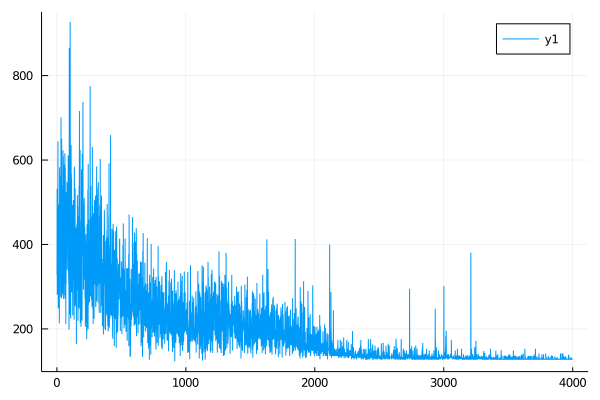
\includegraphics[width=\textwidth]{rews_En3_4k_3layer.png}
    \caption{3 layers trained on a single ideal.}
  \end{subfigure}
  \hfill
  \begin{subfigure}[b]{0.49\textwidth}
    \centering
    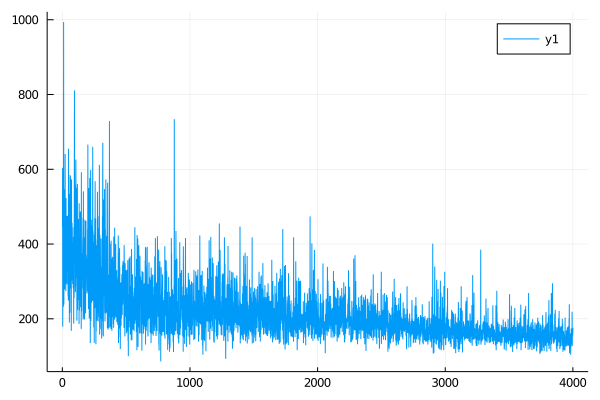
\includegraphics[width=\textwidth]{rews_En3_4k_2layer.png}
    \caption{2 layers trained on a single ideal.}
  \end{subfigure}
  \caption{Comparison of model sizes when training on a single ideal.}
  \label{fig:single_ideal}
\end{figure}


Going up the full training set, we trained the model on dynamically generated ideals. Performance turned out to match the degree strategy but did not exceed it significantly. We theorize this is because we did not implement GAE but instead went with baseline normalization. The results can be seen in table \ref{tab:eval}

\begin{table}
  \centering
  \begin{tabular}{l|rrr}
    Strategy & Random & Degree & Agent \\
    Score    &  398.7 &  219.6 & 206.4
  \end{tabular}
  \caption{Evaluation of the final model trained on random ideals generated by 4 polynomials of degree less than 10 over three variables. Result is average of 1000 random ideals.}
  \label{tab:eval}
\end{table}

The model was trained on 24000 ideals using an ADAM optimizer with a learning rate of $10^{-4}$. We tried finetuning the model by running it for another 8000 iterations with learning rate $10^{-5}$ but this did not improve performance. The training process can be seen in figure \ref{fig:convergence}

\begin{figure}[h]
  \includegraphics[width=0.9\textwidth]{full_24k_En4_2layer.png}
  \caption{Convergence of the neural network. The graph shows a running average of polynomial additions for each network update with window size 1000.}
  \label{fig:convergence}
\end{figure}


\section{Technological choices and demo}
We chose to write the code for this experiment in Julia using the Flux framework for deep learning and building the ReinforcementLearning.jl project as a skeleton for reinforcement learning.

Writing the program in julia had two advantages: we could keep all the code in a single language and we improved running time significantly over the implementation by \cite{peifer}.

Taking a look at \url{https://github.com/dylanpeifer/deepgroebner} we see that $\sim 25\%$ of the project is written in C++. This is an implementation of the Buchberger algorithm and code supporting that and it's nescesary to keep the code fast. However, a TensorFlow model is built in Python and they must use Python code to bridge between TensorFlow and the custom Buchberger code, even though both are written in C++. This incurs a cost, both on the programmer who needs to learn two languages, and on the runtime. Converting between Python and C++ is not free and since this exchange needs to happen at each selection, taking approximately 100 selections to produce a Gröbner basis, this cross-over happens about 8.000.000 times during a training run.

By keeping everything in Julia, which is very fast language, we only need to learn a single language, and we prevent the overhead. In practice, this means that we can train the same models as they did in similar timeframes, but on an Intel i5 CPU instead of an c5n.xlarge AWS instance.

\begin{minted}[breaklines, escapeinside=||, mathescape=true, linenos, numbersep=3pt, gobble=2, frame=lines, fontsize=\small, framesep=2mm]{julia}
  using Deepgroebner
  params = GroebnerEnvParams(3, 10, 4, nothing)
  e = pg_experiment(params, 120_000, 10^-4)
  run(e)

  eval_model(m_pg.env, strat_rand)
  eval_model(m_pg.env, strat_degree)
  eval_model(m_pg.env, m_pg.policy)
\end{minted}








\printbibliography

\end{document}
